\documentclass[fleqn, 11pt]{article}

\usepackage{ucs}
\usepackage[utf8]{inputenc}
\usepackage{babel}
\usepackage{fontenc}
\usepackage{graphicx}
\usepackage{listings}
\usepackage{qtree}
\usepackage{setspace}
\usepackage[margin=5em]{geometry}
\usepackage{amssymb}
\usepackage{amsmath}
\usepackage{esint}
\usepackage{wasysym}
\usepackage[labelformat=empty]{caption}

\date{17/09/2018}

\begin{document}
{\Large CUDA Programming MA5615, Assignment 1}\par
{\small Shaaz Ahmed}, {\small ahmeds1@tcd.ie}, {\small 2018-2019} \par
{\ }\par

\textbf{Answers:} \par
\begin{enumerate}
 \item \textbf{Task 1}:  The code can be found in \texttt{./single\_precision/cpu.cu}. Plotting the execution time in ms against the matrix size, we get the following graph (block size is irrelevant).
\begin{figure}[h]
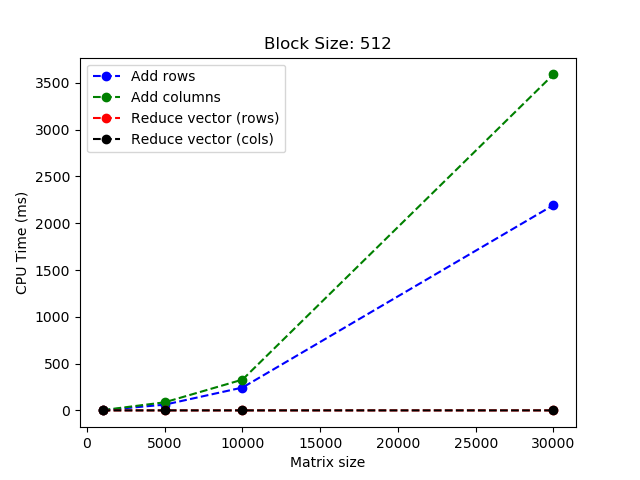
\includegraphics[height=7cm, width=8cm]{../single_precision/time_graphs/time_cpu_512.png}
\centering 
\caption*{{\tiny To generate this graph, uncomment the plotting line from ./run.py and run ./run.py in a GPU supported environment}}
\end{figure} 

It is evident that for both  \texttt{add\_rows} and the \texttt{add\_columns}  the time taken increases significantly as matrix size increases, while this is much less so for the \texttt{reduce\_vector}. This is due to the quadratic complexity nature of \texttt{add\_rows} and \texttt{add\_columns}, while \texttt{reduce\_vector}'s running time grows linearly with matrix size.

Also worth noting that \texttt{add\_rows} is faster than \texttt{add\_columns} (possibly by a factor) - this is because of the better data locality for \texttt{add\_rows} as the elements of rows that have to be summed are close to each other in memory.

 \item \textbf{Task 2}:  The code can be found in \texttt{./single\_precision/gpu.cu}. Plotting the execution time in ms against the matrix size for a block size of 512, we get the following graph.
 
\begin{figure}[h]
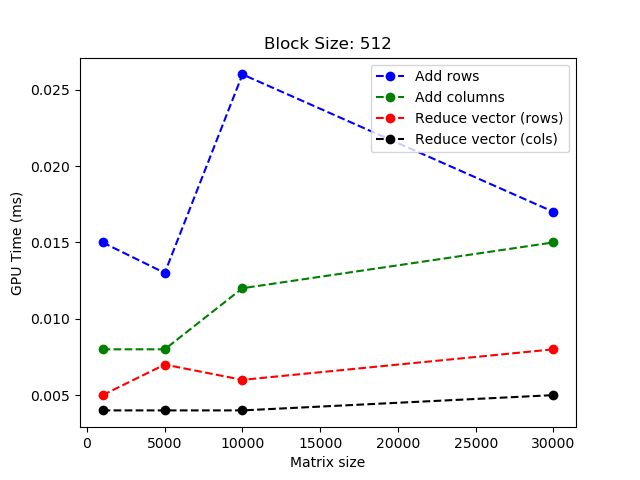
\includegraphics[height=5cm, width=6cm]{../single_precision/time_graphs/time_gpu_512.png}
\centering 
\caption*{{\tiny To generate this graph, uncomment the plotting line from ./run.py and run ./run.py in a GPU supported environment}}
\end{figure} 
\par

This is clearly orders of magnitude faster and the quadratic operations don't seem to behave like they are quadratic anymore.

 \item \textbf{Task 3}:  The speedup graphs for each block size are in \texttt{./single\_precision/speedup\_graphs}. Plotting the speedup against the matrix size for a block size of 512, we get the following graph:
 
\begin{figure}[h]
\includegraphics[height=9cm, width=10cm]{../single_precision/speedup_graphs/speedup_512.png}
\centering 
\caption*{{\tiny To generate this graph, uncomment the plotting line from ./run.py and run ./run.py in a GPU supported environment}}
\end{figure} 
\par
On the specific system this was run on, running NVIDIA GP107M [GeForce GTX 1050 Ti Mobile],  the following are the features of the speedup:
 \begin{itemize}
        \item \texttt{reduce\_vectors} doesn't have much of a speedup because we've used only GPU thread to sum it up. Since the sum has to be stored in a single variable, only one GPU thread can write to it due to consistency issues, or access to the variable has to be serialized, in which case it's almost equivalent in performance to a single thread writing to it - potentially worse.
        
        It is also possible to write this function to use more GPU threads, by splitting the array into evenly-sized sections and summing them separately, using a barrier to synchronize each stage of computation and then further sum their results. This can potentially give a constant factor improvement in performance in the case of large arrays.
        
        \item \texttt{add\_columns} and \texttt{add\_rows} have very large speedups that gets better with matrix size, but the speedup of \texttt{add\_rows} is lesser than that of \texttt{add\_columns} because the CPU  version of \texttt{add\_rows} is slightly faster due to data locality.
        
        \item The block size doesn't seem to affect the speedup significantly on the system that this code was run on (which has a maximum of 1024 threads per block dimension allowed).

Hence, add\_rows and add\_columns are both worth computing using CUDA, which reduce\_vector doesn't have a similar speedup.
        
\end{itemize}
       

 \item \textbf{Task 4}:  The code for double precision and the speedup graphs for each block size are in \texttt{./double\_precision/}, with a similar code structure.  For a block size of 512, the speedup graph is given below.
       
\begin{figure}[h]
\includegraphics[height=9cm, width=10cm]{../double_precision/speedup_graphs/speedup_512.png}
\centering 
\caption*{{\tiny To generate this graph, uncomment the plotting line from ./run.py and run ./run.py in a GPU supported environment}}
\end{figure} 
\par

The following features are noticeable:
\begin{itemize}
 \item The speedup for each of the quadratic operations is much lower than that in the case of single precision arithmetic - nearly an order of magnitude of smaller.
 \item The block size does affect the speedup - the larger the number of blocks, the higher the speedup, as evident from the graphs.
\end{itemize}


\end{enumerate}

\end{document}
